%
% Copyright 2018 Joel Feldman, Andrew Rechnitzer and Elyse Yeager.
% This work is licensed under a Creative Commons Attribution-NonCommercial-ShareAlike 4.0 International License.
% https://creativecommons.org/licenses/by-nc-sa/4.0/
%
\questionheader{ex:s2.6}
%%%%%%%%%%%%%%%%%%
\subsection*{\Conceptual}
%%%%%%%%%%%%%%%%%%

\begin{Mquestion} Spot and correct the error(s) in the following calculation.
\begin{align*}
f(x)&=\frac{2x}{x+1}\\
f'(x)&=\frac{2(x+1)+2x}{(x+1)^2}\\
&=\frac{2(x+1)}{(x+1)^2}\\
&=\frac{2}{x+1}
\end{align*}
\end{Mquestion}
\begin{hint}  Check signs
\end{hint}
\begin{answer}   In the quotient rule, there is a minus, not a plus. Also, $2(x+1)+2x$ is not the same as $2(x+1)$.

 The correct version is:
\begin{align*}
f(x)&=\frac{2x}{x+1}\\
f'(x)&=\frac{2(x+1)\textcolor{red}{-}2x}{(x+1)^2}\\
&=\frac{2}{(x+1)^2}
\end{align*}
\end{answer}
\begin{solution}  In the quotient rule, there is a minus, not a plus. Also, $2(x+1)+2x$ is not the same as $2(x+1)$.

 The correct version is:
\begin{align*}
f(x)&=\frac{2x}{x+1}\\
f'(x)&=\frac{2(x+1)\textcolor{red}{-}2x}{(x+1)^2}\\
&=\frac{2}{(x+1)^2}
\end{align*}
\end{solution}

\begin{Mquestion}
True or false: $\ds\diff{}{x}\{2^x\}=x2^{x-1}$.
\end{Mquestion}
\begin{hint} Read Lemma~\ref*{lem dxn} carefully.
\end{hint}
\begin{answer} False
\end{answer}
\begin{solution}
False: Lemma~\ref*{lem dxn} tells us that, for a constant $n$, $\ds\diff{}{x}\{x^n\}=nx^{n-1}$. Note that the base $x$ is the variable and the exponent $n$ is a constant. In the equation given in the question, the base $2$ is a constant, and the exponent $x$ is the variable: this is the opposite of the situation where Lemma~\ref*{lem dxn} applies.

We do not yet know how to differentiate $2^x$. We'll learn about it in Section~\ref*{sec exp func}.
\end{solution}


%%%%%%%%%%%%%%%%%%
\subsection*{\Procedural}
%%%%%%%%%%%%%%%%%%



\begin{question} Differentiate
$f(x)=\frac{2}{3}x^6+5x^4+12x^2+9$ and factor the result.
\end{question}
\begin{hint} First, factor an $x$ out of the derivative. What's left over looks like a quadratic equation, if you take $x^2$ to be your variable, instead of $x$.
\end{hint}
\begin{answer} $4x(x^2+2)(x^2+3)$
\end{answer}
\begin{solution}
$f(x)=\frac{2}{3}x^6+5x^4+12x^2+9$ is a polynomial:
\begin{align*}
f'(x)&=4x^5+20x^3+24x\\&
=4x(x^4+5x^2+6)\\& = 4x((x^2)^2+5(x^2)+6)\\&=4x(x^2+2)(x^2+3)
\end{align*}
\end{solution}


\begin{question} Differentiate $s(t)=3t^4+5t^3-\frac{1}{t}$.
\end{question}
\begin{hint}
$\frac{1}{t}=t^{-1}$
\end{hint}
\begin{answer} $12t^3+15t^2+\frac{1}{t^2}$
\end{answer}
\begin{solution}  We can rewrite slightly to make every term into a power of $t$:
\begin{align*}
s(t)&=3t^4+5t^3-t^{-1}\\
s'(t)&=4\cdot 3t^{3}+3\cdot 5t^2-(-1)\cdot t^{-2}\\
&=12t^3+15t^2+\frac{1}{t^2}
\end{align*}
\end{solution}



\begin{Mquestion} Differentiate $x(y) = \left(2y+\frac{1}{y}\right)\cdot y^3$.
\end{Mquestion}
\begin{hint} First simplify. Don't be confused by the role reversal of $x$ and $y$: $x$ is just
        the name of the function $\big(2y+\tfrac{1}{y}\big)\cdot y^3$, which
        is a function of the variable $y$. You are to differentiate with
        respect to $y$.
\end{hint}
\begin{answer} $x'(y)=8y^3+2y$
\end{answer}
\begin{solution} We could use the product rule here, but it's easier to simplify first. Don't be confused by the role reversal of $x$ and $y$: $x$ is the name of the function, and $y$ is the variable.
\begin{align*}
x(y) &= \left(2y+\frac{1}{y}\right)\cdot y^3\\
&=2y^4+y^2\\
x'(y)&=8y^3+2y
\end{align*}
\end{solution}


\begin{Mquestion} Differentiate $T(x) = \dfrac{\sqrt{x}+1}{x^2+3}$.
\end{Mquestion}
\begin{hint} $\sqrt{x}=x^{1/2}$
\end{hint}
\begin{answer} $T'(x)=\dfrac{(x^2+3)\left(\frac{1}{2\sqrt{x}}\right)-(\sqrt{x}+1)(2x)}{(x^2+3)^2}$
\end{answer}
\begin{solution}
We've already seen that $\diff{}{x}\{\sqrt{x}\}=\frac{1}{2\sqrt{x}}$, but if you forget this formula it is easy to figure out: $\sqrt{x}=x^{1/2}$, so $\diff{}{x}\{\sqrt{x}\}=\frac{1}{2}x^{-1/2}=\frac{1}{2\sqrt{x}}$.

Using the quotient rule:
\begin{align*}
T(x) &= \dfrac{\sqrt{x}+1}{x^2+3}\\
T'(x)&=\frac{(x^2+3)\left(\frac{1}{2\sqrt{x}}\right)-(\sqrt{x}+1)(2x)}{(x^2+3)^2}
\end{align*}
\end{solution}


\begin{question}[2015Q]
Compute the derivative of $\left(\dfrac{7x+2}{x^2+3}\right)$.
\end{question}
\begin{answer}
$\dfrac{21-4x-7x^2}{(x^2+3)^2}$
\end{answer}
\begin{solution}
We use quotient rule:
\begin{align*}
\frac{(x^2+3)\cdot 7 - 2x\cdot (7x+2)}{(x^2+3)^2}=\frac{21 - 4x - 7x^2}{(x^2+3)^2}
\end{align*}
\end{solution}


\begin{question} What is $f'(0)$, when $f(x)=(3x^3+4x^2+x+1)(2x+5)$?
\end{question}
\begin{hint} You don't need to multiply through.
\end{hint}
\begin{answer} 7
\end{answer}
\begin{solution} Instead of multiplying to get our usual form of this polynomial, we can use the product rule. If $f_1(x)=3x^3+4x^2+x+1$ and $f_2(x)=2x+5$, then\\ $f_1'(x)=9x^2+8x+1$ and $f_2'(x)=2$. Then
\begin{align*}
f'(0)&=f_1'(0)f_2(0)+f_1(0)f_2'(0)\\
&=(1)(5)+(1)(2)=7\end{align*}
\end{solution}


\begin{question} Differentiate $f(x)=\dfrac{3x^3+1}{x^2+5x}$.
\end{question}
\begin{hint} You can use the quotient rule.
\end{hint}
\begin{answer} $\dfrac{3x^4+30x^3-2x-5}{(x^2+5x)^2}
$
\end{answer}
\begin{solution} Using the quotient rule,
\[f'(x) = \frac{(x^2+5x)(9x^2)-(3x^3+1)(2x+5)}{(x^2+5x)^2}
= \frac{3x^4+30x^3-2x-5}{(x^2+5x)^2}
\]\end{solution}


\begin{question} [2015Q]
Compute the derivative of $\left(\dfrac{3x^2+5}{2-x}\right)$
\end{question}
\begin{answer} $\dfrac{-3x^2+12x+5}{(2-x)^2}$
\end{answer}
\begin{solution}
We use quotient rule:
\begin{align*}
\frac{(2-x)(6x)-(3x^2+5)(-1)}{(2-x)^2}=\frac{-3x^2+12x+5}{(x-2)^2}
\end{align*}
\end{solution}


\begin{question}[2015Q]
Compute the derivative of $\left(\dfrac{2-x^2}{3x^2+5}\right)$.
\end{question}
\begin{answer} $\dfrac{-22x}{(3x^2+5)^2}$
\end{answer}
\begin{solution}
We use quotient rule:
\begin{align*}
\frac{(3x^2+5)(-2x) - (2-x^2)(6x)}{(3x^2+5)^2}=\frac{-22x}{(3x^2+5)^2}
\end{align*}
\end{solution}



\begin{question}[2015Q]
 Compute the derivative of $\left(\dfrac{2x^3+1}{x+2}\right)$.
\end{question}
\begin{answer}
$\dfrac{4x^3+12x^2-1}{(x+2)^2}$
\end{answer}
\begin{solution}
We use quotient rule:
\begin{align*}
\frac{6x^2\cdot (x+2)-(2x^3+1)\cdot 1}{(x+2)^2}=\frac{4x^3+12x^2-1}{(x+2)^2}
\end{align*}
\end{solution}




\begin{Mquestion}[2015Q]
For what values of $x$ does the derivative of
$\dfrac{\sqrt{x}}{1-x^2}$ exist? Explain your answer.
\end{Mquestion}
\begin{hint} There are two pieces of the given function that could cause problems.
\end{hint}
\begin{answer}
The derivative of the function is
\begin{align*}
 \frac{(1-x^2)\cdot\frac{1}{2\sqrt{x}} - \sqrt{x} \cdot (-2x)}{(1-x^2)^2}
  &= \frac{(1-x^2) - 2x \cdot (-2x)}{2\sqrt{x}(1-x^2)^2}
\end{align*}
The derivative is undefined if either $x<0$ or $x = 0,\pm 1$ (since the square-root is
undefined for $x<0$ and the denominator is zero when $x=0,1,-1$. Putting this together
--- the derivative exists for $x>0, x\neq 1$.
\end{answer}
\begin{solution}
The derivative of the function is
\begin{align*}
 \frac{(1-x^2)\cdot\frac{1}{2\sqrt{x}} - \sqrt{x} \cdot (-2x)}{(1-x^2)^2}
  &= \frac{(1-x^2) - 2x \cdot (-2x)}{2\sqrt{x}(1-x^2)^2}
\end{align*}
The derivative is undefined if either $x<0$ or $x = 0,\pm 1$ (since the square-root is
undefined for $x<0$ and the denominator is zero when $x=0,1,-1$. Putting this together
--- the derivative exists for $x>0, x\neq 1$.
\end{solution}


\begin{question} Differentiate $f(x)=\left(3\sqrt[5]{x}+15\sqrt[3]{x}+8\right)\left(3x^2+8x-5\right)$.
\end{question}
\begin{hint} $\sqrt[3]{x}=x^{1/3}$
\end{hint}
\begin{answer} $\left(\frac{3}{5}{x}^{\frac{-4}{5}}+5{x}^{\frac{-2}{3}}\right)\left(3x^2+8x-5\right)+
\left(3\sqrt[5]{x}+15\sqrt[3]{x}+8\right)\left(6x+8\right)$
\end{answer}
\begin{solution} Using the product rule seems faster than expanding.
\begin{align*}
f'(x)&=\diff{}{x}\left\{3\sqrt[5]{x}+15\sqrt[3]{x}+8\right\}\left(3x^2+8x-5\right)+
\left(3\sqrt[5]{x}+15\sqrt[3]{x}+8\right)\diff{}{x}\left\{3x^2+8x-5\right\}\\
&=\diff{}{x}\left\{3{x}^{\frac{1}{5}}+15{x}^{\frac{1}{3}}+8\right\}\left(3x^2+8x-5\right)+
\left(3\sqrt[5]{x}+15\sqrt[3]{x}+8\right)\diff{}{x}\left\{3x^2+8x-5\right\}\\
&=\left(\frac{3}{5}{x}^{\frac{-4}{5}}+5{x}^{\frac{-2}{3}}\right)\left(3x^2+8x-5\right)+
\left(3\sqrt[5]{x}+15\sqrt[3]{x}+8\right)\left(6x+8\right)
\end{align*}
\end{solution}

\begin{question} Differentiate $f(x)=\dfrac{(x^2+5x+1)(\sqrt{x}+\sqrt[3]{x})}{x}$.
\end{question}
\begin{hint} Simplify first
\end{hint}
\begin{answer} $f'(x)=(2x+5)(x^{-1/2}+x^{-2/3})+(x^2+5x+1)\left(\frac{-1}{2}x^{-3/2}-\frac{2}{3}x^{-5/3}\right)$
\end{answer}
\begin{solution} To avoid the quotient rule, we can divide through the denominator:
\begin{align*}
f(x)&=\dfrac{(x^2+5x+1)(\sqrt{x}+\sqrt[3]{x})}{x}
=(x^2+5x+1)\dfrac{(\sqrt{x}+\sqrt[3]{x})}{x}\\
&=(x^2+5x+1)(x^{-1/2}+x^{-2/3})
\intertext{Now, product rule:}
f'(x)&=(2x+5)(x^{-1/2}+x^{-2/3})+(x^2+5x+1)\left(\frac{-1}{2}x^{-3/2}-\frac{2}{3}x^{-5/3}\right)
\end{align*}
(If you simplified differently, or used the quotient rule, you probably came up with a different-looking answer. There is only one derivative, though, so all correct answers will look the same after sufficient algebraic manipulation.)
\end{solution}

\begin{Mquestion} Find all $x$-values where $f(x)=\dfrac{1}{\frac{1}{5}x^5+x^4-\frac{5}{3}x^3}$ has a horizontal tangent line.
\end{Mquestion}
\begin{answer} $x=-5$ and $x=1$
\end{answer}
\begin{solution}
The question asks us to find where $f'(x)=0$ and $f(x)$ exists. We can use the formula for the derivative of a reciprocal, Corollary~\ref*{cor diff recip}:
\begin{align*}
f'(x) &= \frac{-\diff{}{x}\left\{\frac{1}{5}x^5+x^4-\frac{5}{3}x^3\right\}}{\left(\frac{1}{5}x^5+x^4-\frac{5}{3}x^3\right)^2}\\
&=\frac{-\left(x^4+4x^3-{5}x^2\right)}{\left(\frac{1}{5}x^5+x^4-\frac{5}{3}x^3\right)^2}\\
&=\frac{-x^2\left(x^2+4x-{5}\right)}{\left(\frac{1}{5}x^5+x^4-\frac{5}{3}x^3\right)^2}\\
&=\frac{-x^2(x+5)(x-1)}{\left(\frac{1}{5}x^5+x^4-\frac{5}{3}x^3\right)^2}
\end{align*}
So our candidates for $x$-values where $f'(x)=0$ are $x=0$, $x=-5$, and $x=1$. However, we need to check that $f$ exists at these places:  $f(0)$ is undefined (and  $f'(0)$ doesn't exist). So $f'(x)=0$ only when $x=-5$ and $x=1$.
\end{solution}

%%%%%%%%%%%%%%%%%%
\subsection*{\Application}
%%%%%%%%%%%%%%%%%%



\begin{question}[2007H]
 Find an equation of a line that is tangent to both of the
curves $y = x^2$ and $y = x^2 - 2x + 2$ (at different points).
\end{question}
\begin{hint}
Let $m$ be the slope of such a tangent line, and let $P_1$ and $P_2$ be the points where the tangent line is tangent to the two curves, respectively. There are three equations $m$ fulfils: it has the same slope as the curves at the given points, and it is the slope of the line passing through the points $P_1$ and $P_2$.
\end{hint}
\begin{answer}
 $y=x-\dfrac{1}{4}$
\end{answer}
\begin{solution}
Denote by $m$ the slope of the common tangent, by $(x_1,y_1)$
the point of tangency with $y=x^2$, and by $(x_2,y_2)$ the point of tangency
with $y=x^2-2x+2$. Then we must have
$$
y_1=x_1^2\qquad
y_2=x_2^2-2x_2+2\qquad
m=2x_1=2x_2-2=\frac{y_2-y_1}{x_2-x_1}
$$
From the ``$m$'' equations we get $x_1=\frac{m}{2}$, $x_2=\frac{m}{2}+1$
and
\begin{align*}
m&=\frac{y_2-y_1}{x_2-x_1}\\
&=y_2-y_1\\
&=x_2^2-2x_2+2-x_1^2\\
\\& =(x_2-x_1)(x_2+x_1)-2(x_2-1)\\
&=\left(\frac{m}{2}+1-\frac{m}{2}\right)\left(\frac{m}{2}+1+\frac{m}{2}\right)
-2\left(\frac{m}{2}+1-1\right)
\\ &=(1)(m+1)-2\frac{m}{2}\\
 &=1\\
\mbox{So,}~~~m&=1,\qquad
x_1=\half,\qquad
y_1=\frac{1}{4},\qquad
x_2=\frac{3}{2},\qquad
y_2=\frac{9}{4}-3+2=\frac{5}{4}
\end{align*}
An equation of the common tangent is $y=x-\frac{1}{4}$.
\end{solution}



\begin{Mquestion} [1998H]
Find all lines that are tangent to both of the curves $y=x^2$
and $y=-x^2+2x-5$. Illustrate your answer with a sketch.
\end{Mquestion}
\begin{hint} A line has equation $y=mx+b$, for some constants $m$ and $b$.
 What has to be true for $y=mb+x$ to be tangent to the first curve at the point $x=\alpha$, and to the second at the point $x=\beta$?
\end{hint}
\begin{answer}
\begin{center}
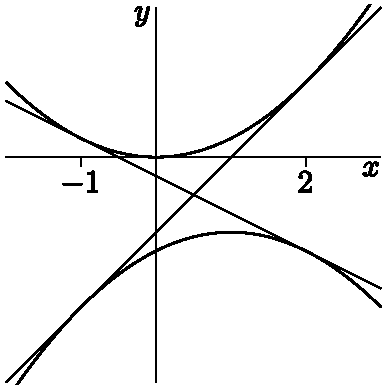
\includegraphics{graphE3c}
\end{center}
$y=4x-4$ and $y=-2x-1$
\end{answer}
\begin{solution}
The line $y=mx+b$ is tangent to $y=x^2$ at $x=\alpha$ if
$$
2\alpha=m\hbox{ and }\alpha^2=m\alpha+b
\iff m=2\alpha\hbox{ and }b=-\alpha^2
$$
The same line $y=mx+b$ is tangent to $y=-x^2+2x-5$ at $x=\beta$ if
\begin{align*}
-2\beta+2=m&\hbox{ and }-\beta^2+2\beta-5=m\beta+b\\
\iff m=2-2\beta&\hbox{ and }b=-\beta^2+2\beta-5-(2-2\beta)\beta=\beta^2-5
\end{align*}
For the line to be simultaneously tangent to the two parabolas we need
$$
m=2\alpha=2-2\beta\hbox{ and }b=-\alpha^2=\beta^2-5
$$
Substituting $\alpha=1-\beta$ into $-\alpha^2=\beta^2-5$ gives $-(1-\beta)^2=\beta^2-5$
or $2\beta^2-2\beta-4=0$ or $\beta=-1,2$. The corresponding values of the other
parameters are $\alpha=2,-1$, $m=4,-2$ and $b=-4,-1$. The two lines are
{$y=4x-4$ and $y=-2x-1$}.
\begin{center}
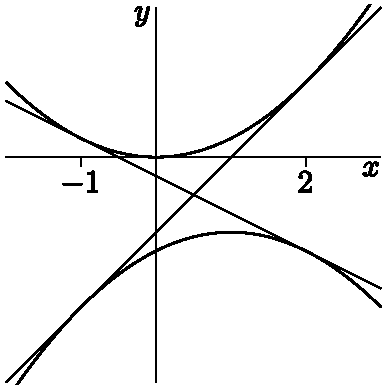
\includegraphics{graphE3c}
\end{center}
\end{solution}



\begin{question}[2015Q]
Evaluate $\displaystyle \lim_{x\to 2}\left(
\dfrac{x^{2015}-2^{2015}}{x-2}\right).$
\end{question}
\begin{hint}
Compare this to one of the forms given in the text for the definition of the derivative.
\end{hint}
\begin{answer}
{$2015\cdot 2^{2014}$}
\end{answer}
\begin{solution}
This limit represents the derivative computed at $x=2$ of the function $f(x)=x^{2015}$.
To see this, simply use the definition of the derivative at $a=2$ with $f(x)=x^{2015}$:
\begin{align*}
\left.\diff{}{x}\{f(x)\}\right|_{a} &= \lim_{x \to a}\frac{f(x)-f(a)}{x-a}\\
\left.\diff{}{x}\{x^{2015}\}\right|_{2} &=\lim_{x\to2} \frac{x^{2015}-2^{2015}}{x-2}
\end{align*}
Since the derivative of $f(x)$ is $2015\cdot x^{2014}$, then its value at $x=2$ is exactly $2015\cdot 2^{2014}$.
\end{solution}
